\section{Theory}

\begin{figure}[H]    
    \centering
    \begin{circuitikz}[american voltages ]
        \draw
        % Transistor
        (0,0) node[npn, anchor=E, tr circle, fill = cyan!40!white] (Q) {}
        (Q.B) node[above left] {B}
        (Q.C) node[right] {C}
        (Q.E) node[below left] {E}
        % Base resistor
        (Q.B) -- (-2,0.75) to[R, l=$\mathrm{R_B}$] (-4,0.75) to [rmeter, t = $\mathrm{\mu A}$,fill = yellow!60!white]  (-6,0.75)
        to[battery, v_=$\mathrm{V_{BB}}$] (-6,-2) -- (0,-2)
    
        % Collector resistor
        (Q.C) -- (0,2) to[R, l=$\mathrm{R_C}$] (4,2)
        to [rmeter, t= $\mathrm{mA}$, fill = yellow!60!white] (5,2) -- (7,2)
        to [battery, v=$\mathrm{V_{CC}}$] (7,-2) -- (0,-2) 
    
        % Ground connection
        (Q.E) -- (0,-2) node[ground] {};
    \end{circuitikz}   
    \caption{Circuit diagram of a common emitter configuration of a NPN transistor}  
\end{figure}



\subsection{Bipolar Junction Transistor (BJT)}
The Bipolar Junction Transistor (BJT) is essentially a combination of two PN junction diodes.  According to the order in which the diodes are connected, we have npn and pnp transistors. The emitter region is much smaller than the collector and much more strongly doped while the base is very thing and very lightly doped. A large collector is needed since it should have more surface area for dissipating the power generated there.\\[0.3cm]
\begin{figure}[H]
    \centering

\tikzset{every picture/.style={line width=0.75pt}} %set default line width to 0.75pt        

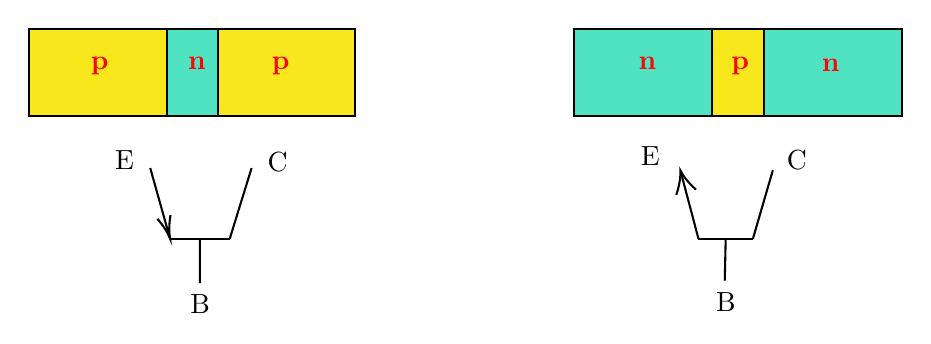
\begin{tikzpicture}[x=0.75pt,y=0.75pt,yscale=-1,xscale=1]
%uncomment if require: \path (0,242); %set diagram left start at 0, and has height of 242

%Shape: Rectangle [id:dp45633474700626153] 
\draw  [fill={rgb, 255:red, 248; green, 231; blue, 28 }  ,fill opacity=1 ] (95.6,52) -- (162.01,52) -- (162.01,94.08) -- (95.6,94.08) -- cycle ;
%Shape: Rectangle [id:dp14383516673441366] 
\draw  [fill={rgb, 255:red, 248; green, 231; blue, 28 }  ,fill opacity=1 ] (186.48,52) -- (252.89,52) -- (252.89,94.08) -- (186.48,94.08) -- cycle ;
%Shape: Rectangle [id:dp555436172774842] 
\draw  [fill={rgb, 255:red, 80; green, 227; blue, 194 }  ,fill opacity=1 ] (162.01,52) -- (186.91,52) -- (186.91,94.08) -- (162.01,94.08) -- cycle ;
%Shape: Rectangle [id:dp25579750012111335] 
\draw  [fill={rgb, 255:red, 80; green, 227; blue, 194 }  ,fill opacity=1 ] (358.45,52) -- (424.86,52) -- (424.86,94.08) -- (358.45,94.08) -- cycle ;
%Shape: Rectangle [id:dp7671828884714951] 
\draw  [fill={rgb, 255:red, 80; green, 227; blue, 194 }  ,fill opacity=1 ] (449.76,52) -- (516.17,52) -- (516.17,94.08) -- (449.76,94.08) -- cycle ;
%Shape: Rectangle [id:dp5338560444707424] 
\draw  [fill={rgb, 255:red, 248; green, 231; blue, 28 }  ,fill opacity=1 ] (424.86,52) -- (449.76,52) -- (449.76,94.08) -- (424.86,94.08) -- cycle ;
%Straight Lines [id:da24796501054461773] 
\draw    (163.72,153.23) -- (192.44,153.23) ;
%Straight Lines [id:da6481562502442813] 
\draw    (163.18,151.3) -- (154.15,119.15) ;
\draw [shift={(163.72,153.23)}, rotate = 254.31] [color={rgb, 255:red, 0; green, 0; blue, 0 }  ][line width=0.75]    (10.93,-3.29) .. controls (6.95,-1.4) and (3.31,-0.3) .. (0,0) .. controls (3.31,0.3) and (6.95,1.4) .. (10.93,3.29)   ;
%Straight Lines [id:da7575975492052729] 
\draw    (192.44,153.23) -- (202.98,119.15) ;
%Straight Lines [id:da35919367940892855] 
\draw    (418.29,153.23) -- (444.51,153.23) ;
%Straight Lines [id:da5671054714723539] 
\draw    (418.29,153.23) -- (410.06,122.13) ;
\draw [shift={(409.55,120.2)}, rotate = 75.18] [color={rgb, 255:red, 0; green, 0; blue, 0 }  ][line width=0.75]    (10.93,-4.9) .. controls (6.95,-2.3) and (3.31,-0.67) .. (0,0) .. controls (3.31,0.67) and (6.95,2.3) .. (10.93,4.9)   ;
%Straight Lines [id:da2022169589051811] 
\draw    (444.51,153.23) -- (454.12,120.2) ;
%Straight Lines [id:da04159202121636396] 
\draw    (178.08,153.23) -- (178.06,174.6) ;
%Straight Lines [id:da31155623971098534] 
\draw    (431.4,153.23) -- (430.96,173.37) ;

% Text Node
\draw (387.97,64.01) node [anchor=north west][inner sep=0.75pt]   [align=left] {\textcolor[rgb]{0.96,0.03,0.03}{\textbf{n}}};
% Text Node
\draw (476.29,65.06) node [anchor=north west][inner sep=0.75pt]   [align=left] {\textcolor[rgb]{0.96,0.03,0.03}{\textbf{n}}};
% Text Node
\draw (170.87,64.01) node [anchor=north west][inner sep=0.75pt]   [align=left] {\textcolor[rgb]{0.96,0.03,0.03}{\textbf{n}}};
% Text Node
\draw (211.31,64.01) node [anchor=north west][inner sep=0.75pt]   [align=left] {\textcolor[rgb]{0.96,0.03,0.03}{\textbf{p}}};
% Text Node
\draw (124.05,64.01) node [anchor=north west][inner sep=0.75pt]   [align=left] {\textcolor[rgb]{0.96,0.03,0.03}{\textbf{p}}};
% Text Node
\draw (432.66,64.01) node [anchor=north west][inner sep=0.75pt]   [align=left] {\textcolor[rgb]{0.96,0.03,0.03}{\textbf{p}}};
% Text Node
\draw (135.79,109.24) node [anchor=north west][inner sep=0.75pt]   [align=left] {E};
% Text Node
\draw (209.25,110.3) node [anchor=north west][inner sep=0.75pt]   [align=left] {C};
% Text Node
\draw (171.97,178.67) node [anchor=north west][inner sep=0.75pt]   [align=left] {B};
% Text Node
\draw (389.06,107.14) node [anchor=north west][inner sep=0.75pt]   [align=left] {E};
% Text Node
\draw (425.24,177.62) node [anchor=north west][inner sep=0.75pt]   [align=left] {B};
% Text Node
\draw (459.33,109.24) node [anchor=north west][inner sep=0.75pt]   [align=left] {C};


\end{tikzpicture}

\end{figure}

\noindent
It is a three terminal device with the terminals named as emitter, base and collector but to act as an amplifier, we need four terminals. Hence, we make one terminal common. The most commonly studied configuration is the common emitter configuration where the emmiter is common to both input and output.\\[0.3cm]
A BJT works in three modes: Active, Saturation and Cutoff Modes, according to which junction is forward or reverse biased. 
\subsection{Common Emitted Configuration of BJT}

Hello world!